\documentclass[uplatex,titlepage]{jsarticle}
%\documentclass{jsarticle}

\usepackage[dvipdfmx]{graphicx}
\usepackage[dvipdfmx]{color}
\usepackage{bm}%数式内の太字
\usepackage{subcaption}

%\title{\vspace{-5cm}パターン情報学 プログラミング課題2}
\title{自主プロジェクトレポート課題}
\author{学生番号03-180255 赤瀬稔尚}
\date{\today}
\begin{document}
\maketitle

\section{ゲームの説明}
自主プロジェクトでにんげんタワーバトルを製作した.
このゲームは有名なスマートフォンアプリのどうぶつタワーバトルを応用して作ったものである.まず,にんげんタワーバトルの説明の前に,どうぶつタワーバトルについて説明をすると,
どうぶつタワーバトルとは,2次元の平面上で出てきた動物を,位置や向きを調整しながら台の上に交互に積み上げていく対戦ゲームである.勝敗は先に台の下に動物を落としたプレイヤーの負けとなるゲームである.(図\ref{doubutu})

にんげんタワーバトルはこのゲームを拡張したものであるが主な変更部分としては,2次元から3次元になったこと,また出てくる動物を人型の人形にしてその人形のポーズを実際のプレイヤーがポーズをとることによって決められることである.
%\begin{figure}[h]
% \begin{minipage}[b]{0.5\linewidth}
%  \centering
%  \includegraphics[keepaspectratio, scale=0.5]
%  {images/doubutu.png}
%  \subcaption{どうぶつタワーバトル}\label{doubutu}
% \end{minipage}
% \begin{minipage}[b]{0.5\linewidth}
%  \centering
%  \includegraphics[keepaspectratio, scale=0.5]
%  {images/ningenn.png}
%  \subcaption{にんげんタワーバトル}\label{ningenn}
% \end{minipage}
% \caption{ゲームの比較画面}
% \label{doubutu1}
%\end{figure}

\begin{figure}
\begin{center}
   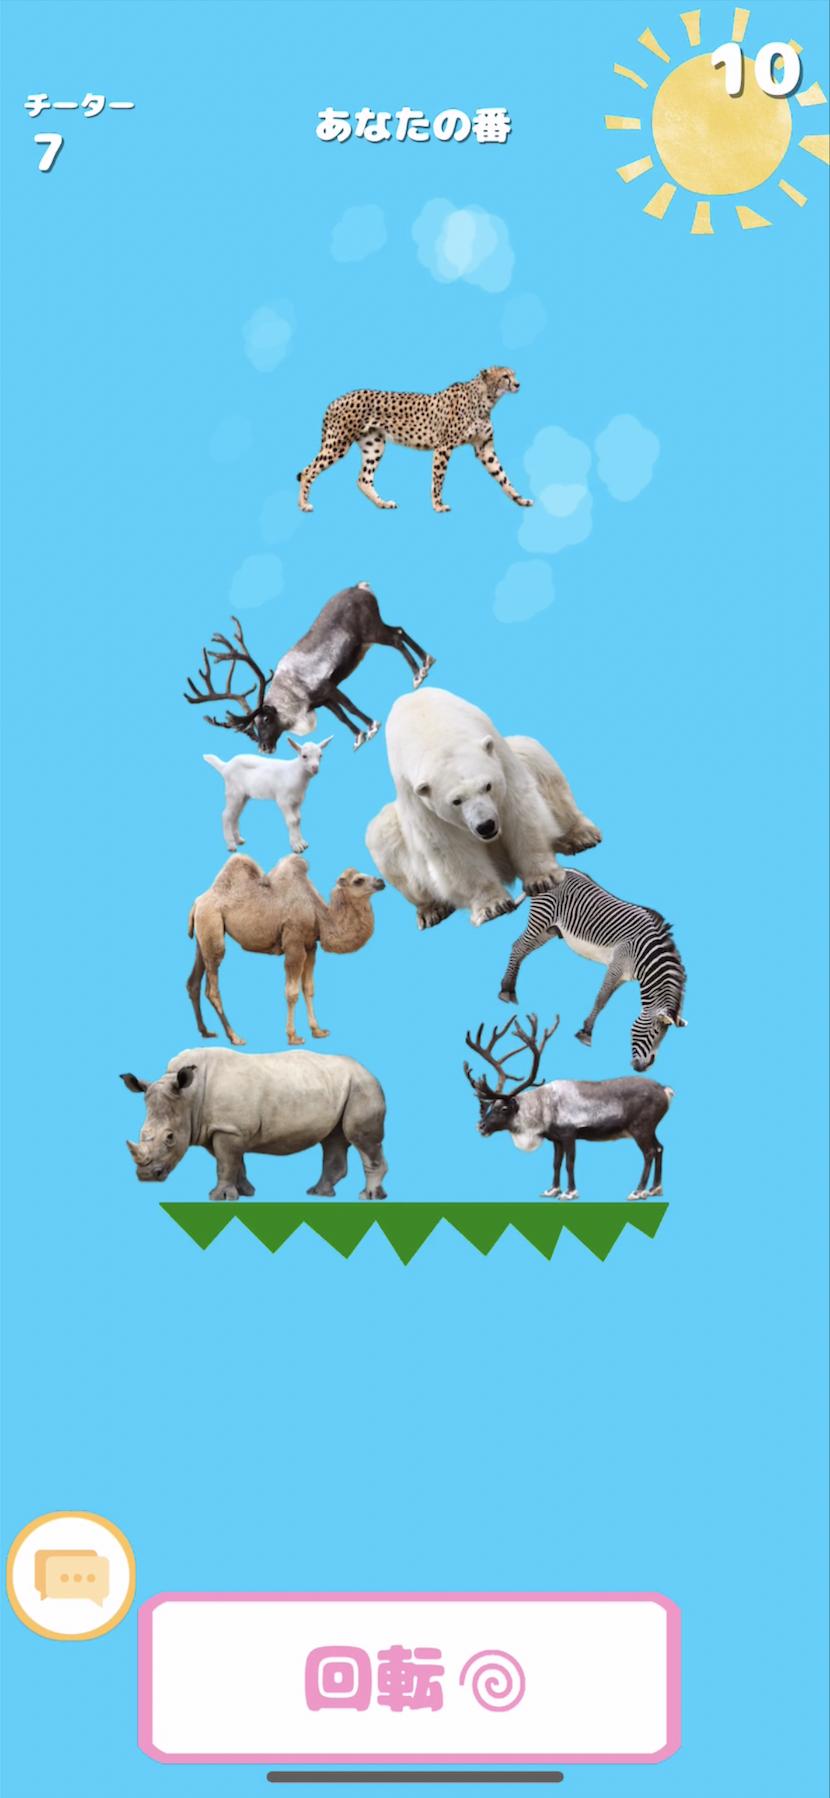
\includegraphics[width=5.0cm]{images/doubutu.PNG}
 \caption{どうぶつタワーバトルのゲーム画面}
 \label{doubutu}
 \end{center}
\end{figure}

\section{実装の説明}
このゲームを作るにあたって,最も重要なものは人のポーズをどのようにして認識するかという問題である.最初はopenpose\cite{openpose}という1枚の写真から骨格を認識しそこから三次元の姿勢を推定するソフトを用いることでその3次元座標をunityにうまく落とし込めるのではないかと考え,openposeを用いて製作を行った.手順としては,まず画像を読み込ませることで,骨格を2次元平面上で認識させ,その認識した骨格を機械学習を用いてさらに3次元情報に変換することにより骨格推定を行っている.
実際,図\ref{openpose}のようにうまく骨格推定はできたのだが,gpuが搭載されていないパソコンで,かつ仮想環境上で処理を行ったため,画像一枚につき処理時間が1分以上かかってしまいゲームに使えないことが判明した.ここで数日取られてしまい大幅に遅れを取ってしまった.

そこで,Kinectを用いることにした.
幸いなことにkinect v2 example with ms-sdk\cite{kinect}(以下,これをkinectアセットと呼ぶ)というkinectで骨格推定を行いそれをモデルの骨格に反映させるという便利なunityのアセットがあったためそれを用いた.骨格推定を行ったあとは,kinectアセットにより人がとったポーズを人形に反映させ,その人形を落とす位置や姿勢を決め重力を与えて落とす,というように後はどうぶつタワーバトルと同じ仕組みになるようにした.
他にも,ポーズを取りながらゲームを実行できるように,wiiリモコンでゲームの操作ができるようにした.(しかし,本番では赤外線センサーバーがなかったためwiiリモコンではなくマウスを用いて行うことになってしまった.)

処理の流れを図\ref{hyou}としてまとめたので,以下これに従って説明を行う.この図のように自分がプログラムしたのは主に
ゲーム画面についてである.
まずは,認識した骨格が反映されたモデルは常にプレイヤーの動きに合わせて動くのだが,ポーズをきめてモデルを落とす時にはプレイヤーの動きが反映されてはいけない(ポーズを固定する)ため,プレイヤーの思い通りのポーズになった時にkinectのアセットとモデルの接続を切り離すことでモデルのポーズが固定されるようにした.簡単そうに見えるが,kinectのスクリプトを理解する必要があったためここで多くの時間を費やしてしまった.
%このkinectから骨格を推定させそれを人形にリンクさせるプログラムは,unityのシーン起動時に実行され,そのクラスで得た情報を人形に当てはめた別のプログラムで読み取りそのデータを人形にリンクさせることで動作させていた.また,そのkinectアセットは

次に,このポーズが固定されたモデルを落とす位置と姿勢を決め,そのモデルに重力を付加して落とす段階なのだが,ここではUnityの関数をうまく用いることで実装することができた.
また,unityには衝突判定の形が立方体や三角錐,円柱など基本的な形しかなかったため,衝突判定がモデルの形に沿うようなポリゴンに変更するというアセットを用いることで実現させた.

%次に落下後の動きが止まったらプレイヤーを変更するという場面についてなのだが,このゲームはものを積み重ねていくゲームなので,モデルを落とす位置は低ければ低いほど有利になってしまうので,落とす高さはプレイヤーに決めさせずに自動で決める必要があった.
%そのため,モデルを落とす高さが積み重なったタワーの最高点から一定の高さになるように決めたのだが.タワーの最高点を求めてくれるような便利な関数は存在しなかったため,自分で実装した.
%実装方法としては,衝突判定を持った平面を徐々に上げていき,平面とタワーとが接触しなくなった点を最高点にすることで実現させた.
%台から落下したかどうかの判定も,このように衝突判定を持つ平面を台の下に設置することで実現させた.
%他にも,どうぶつタワーバトルに寄せたかったため背景を2次元にしたのだが,カメラを回転させると背景の平面もそれに合わせて常にカメラの真反対にいるようにしたりなど,見た目にもこだわった.

これらのステップはシーンを切り替えれば楽に行えると思うのだが,自分が用いたkinectアセットがシーン
を切り替えるとうまく作動してくれないため,すべてシーンの切り替えではなくカメラの切り替えで場面を変更することにした.

%ここから詳細
%以下そのシーンの切り替えについての詳しい説明を行う.
上で述べたようにシーンの切り替えができなかったため全てグローバル変数の値によってカメラの位置などを変更することで,シーンが変化したように見せた.
C\#のクラスを20個作りそれらのクラス間で変数を共有することで,カメラの切り替えなどの全ての機能を実現させた.その中で,
メインとなるクラスについての説明を行うと,
まずカメラの切り替えなどそれぞれの行動をおこす場面をメインクラスの中のグローバル変数を利用して作成し,
整数の0,1,2,3,4の値で表現した.0の時は,人形が落ちているのを確認する段階,1の時は落とすモデルのポーズを決める段階,2の時はポーズを決めたモデルを落とす台の上に生成する段階,3の時は落とす位置と姿勢を決める段階,4はそのモデルに重力を付加することで落とし,落下後に人形のタワーが静止するまで見る段階とした.場面の切り替えは,主に画面上にあるボタンがクリックされた時に行われるようにし,一部の場面遷移に,人形のタワーが静止したことを別のクラスで認識しその静止状態を用いることで実現させた.
カメラは3つ存在し,メインとなるタワーを積み重ねる台を横から見るためのカメラ(main camera),落とす位置がわかりやすいように台を真上から見るカメラ(overlook camera),落とすモデルのポーズを決めるカメラ(other camera)の3つを用意し,main cameraは全ての場面で利用し,other cameraは場面1で,overlook cameraは場面3で利用した.
1つの場面で2つのカメラを利用する時は,縦に6:4の比で2つの画面を並べた.
overlook cameraに関しては落とす位置がわかりやすいように,視線が平行の平行投影カメラを用い,他のカメラは,距離感がわかるように透視投影カメラを用いた.

まず,落とす位置に関してはunityのgameobject.transform.positionを利用し変更させ,落とす位置が決まると次の場面に切り替えかえるのだが,場面が切り替わると次に落とす位置が元の位置になるように位置の値をリセットさせた.
また,人形の姿勢(ポーズではない)に関しては,大きい半径を持つ球殻上の点をボタン入力によって移動させunityのgameobject.transform.lookatを用いてモデルにその点の方向を向かせることで,姿勢を調整させた.また,これだけでは全自由度が表せていない(モデルの背骨を軸とした回転が表せていない)ので,unityのgameobject.transform.rotatearound()関数に,モデルの中心座標,回転軸のベクトル,回転量を入力することで,モデルの姿勢が全ての方向が向けるように実現させた.これも,落とす位置を決めるのと同じく,実際に落とし始めたら次の落とすモデルに影響が出ないように初期化させた.

落下判定に関しては,台の下に透明な大きな平面を作成することで,モデルとその平面が衝突したかどうかにより判定を行った.
また,モデルを落とす位置に関してなのだが,ゲームの性質上,上で述べたモデルの落とす水平位置や姿勢はプレイヤーに決めさせてもいいが,落とす高さに関してはゲーム上で勝手に決める必要があった.(落とす高さは低ければ低いほど有利になるため.)
そのため,台の少し上に透明な大きな平面を作成しその平面と台の上に積み上がったモデルとの衝突判定を常に確認し,衝突判定がなくなるまで透明な平面の高度をあげることで,透明な平面の高さが積み重なったタワーの最高点の高さを求めた.あとはそれを利用し,求めた最高点の高さから一定の高さを加えた値を,モデルを落とす位置とした.この最高点の高さはmain cameraの高さの座標にも利用した.
上で利用した場面を表すグローバル変数は,画面上にコメントをつけたり,プレイヤーの表示を切り替えたりなどにも利用した.

他に工夫した点として,今回のゲームはどうぶつタワーバトルに似せようとしたため,3次元空間上でのゲームとなってはいるものの背景は2次元の背景にしたかった.main cameraの機能にはタワーを積み上げる台を360度全ての方向から見えるようにしたため,2次元背景を置く位置を固定してしまうとカメラの移動に伴い背景が変になってしまう(横から平面を見たようになってしまう)ため,カメラの動きに合わせ背景も台の中央を中心とした点に関して常に点対称に動くように調整することで背景が綺麗に表示させるようにした.



そのため,図\ref{hyou}の各ステップごとに画面の遷移が必要なため,意外とカメラの動きや,場面ごとに変わる使うカメラの切り替えなどのプログラムを記述するのが大変であった.
\begin{figure}
\begin{center}
   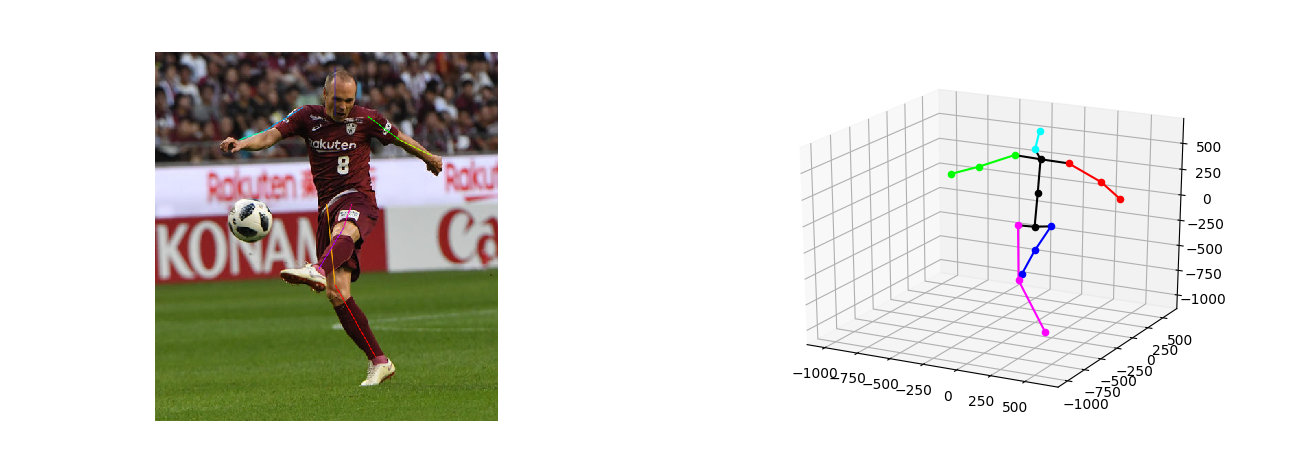
\includegraphics[width=15.0cm]{images/openpose.png}
 \caption{openposeの実行画面}
 \label{openpose}
 \end{center}
\end{figure}

\begin{figure}
\begin{center}
   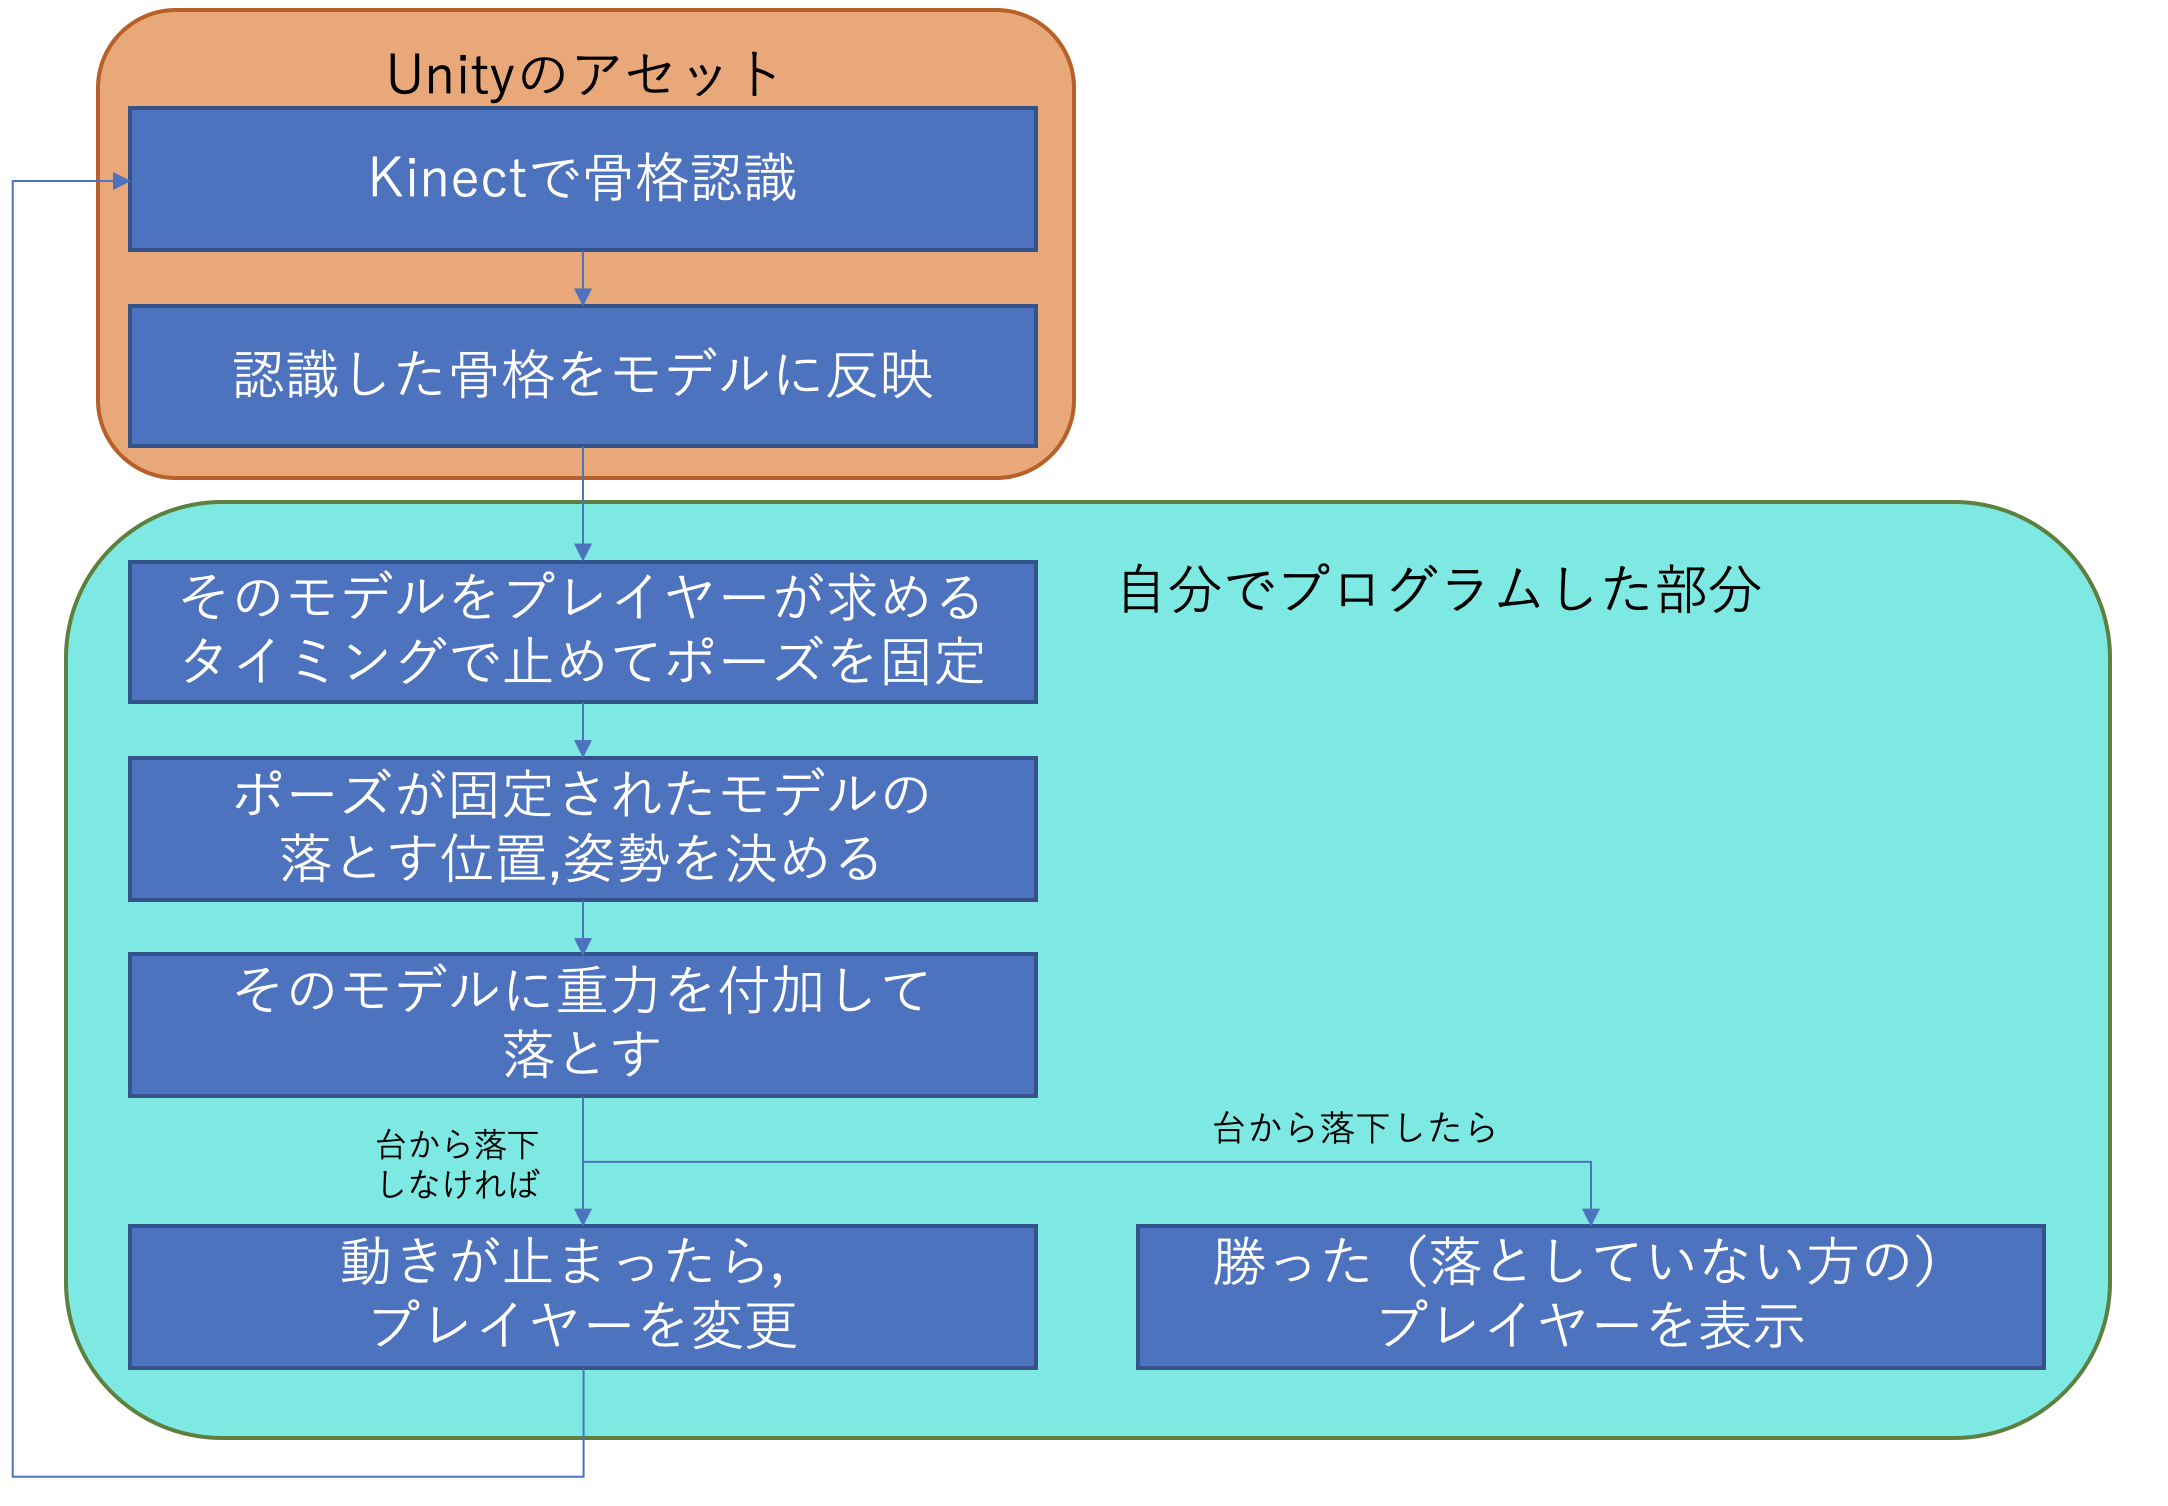
\includegraphics[width=10.0cm]{images/hyou.png}
 \caption{大まかな処理の流れ}
 \label{hyou}
 \end{center}
\end{figure}

\section{ゲーム画面}
図\ref{start}はスタート画面で,どうぶつタワーバトルによせた.この図の中にある丸い点がwiiリモコンのカーソルとなっており,wiiリモコンで操作をすることができる.
図\ref{pose}はポーズを決める画面で,画面右には台の映像がありその台の様子を見ながら(この写真ではまだ何も載っていないが)ポーズを決めることができる.
図\ref{position1},\ref{position2}は姿勢や位置を決める画面であり,画面右で落とす水平位置を決め,画面右で落とす姿勢を決めることができる.ここでは,ちゃんと姿勢は3次元すべての角度の状態を表せるように
した.
図\ref{tumi}は積み重ねていった画面で,この画面では初期姿勢のまま積み重ねていったがこのようにどんどん積み重ねていくことができる.自分がやった中では10体以上積み重ねて遊ぶことができた.

\begin{figure}[h]
 \begin{minipage}[b]{0.5\linewidth}
  \centering
  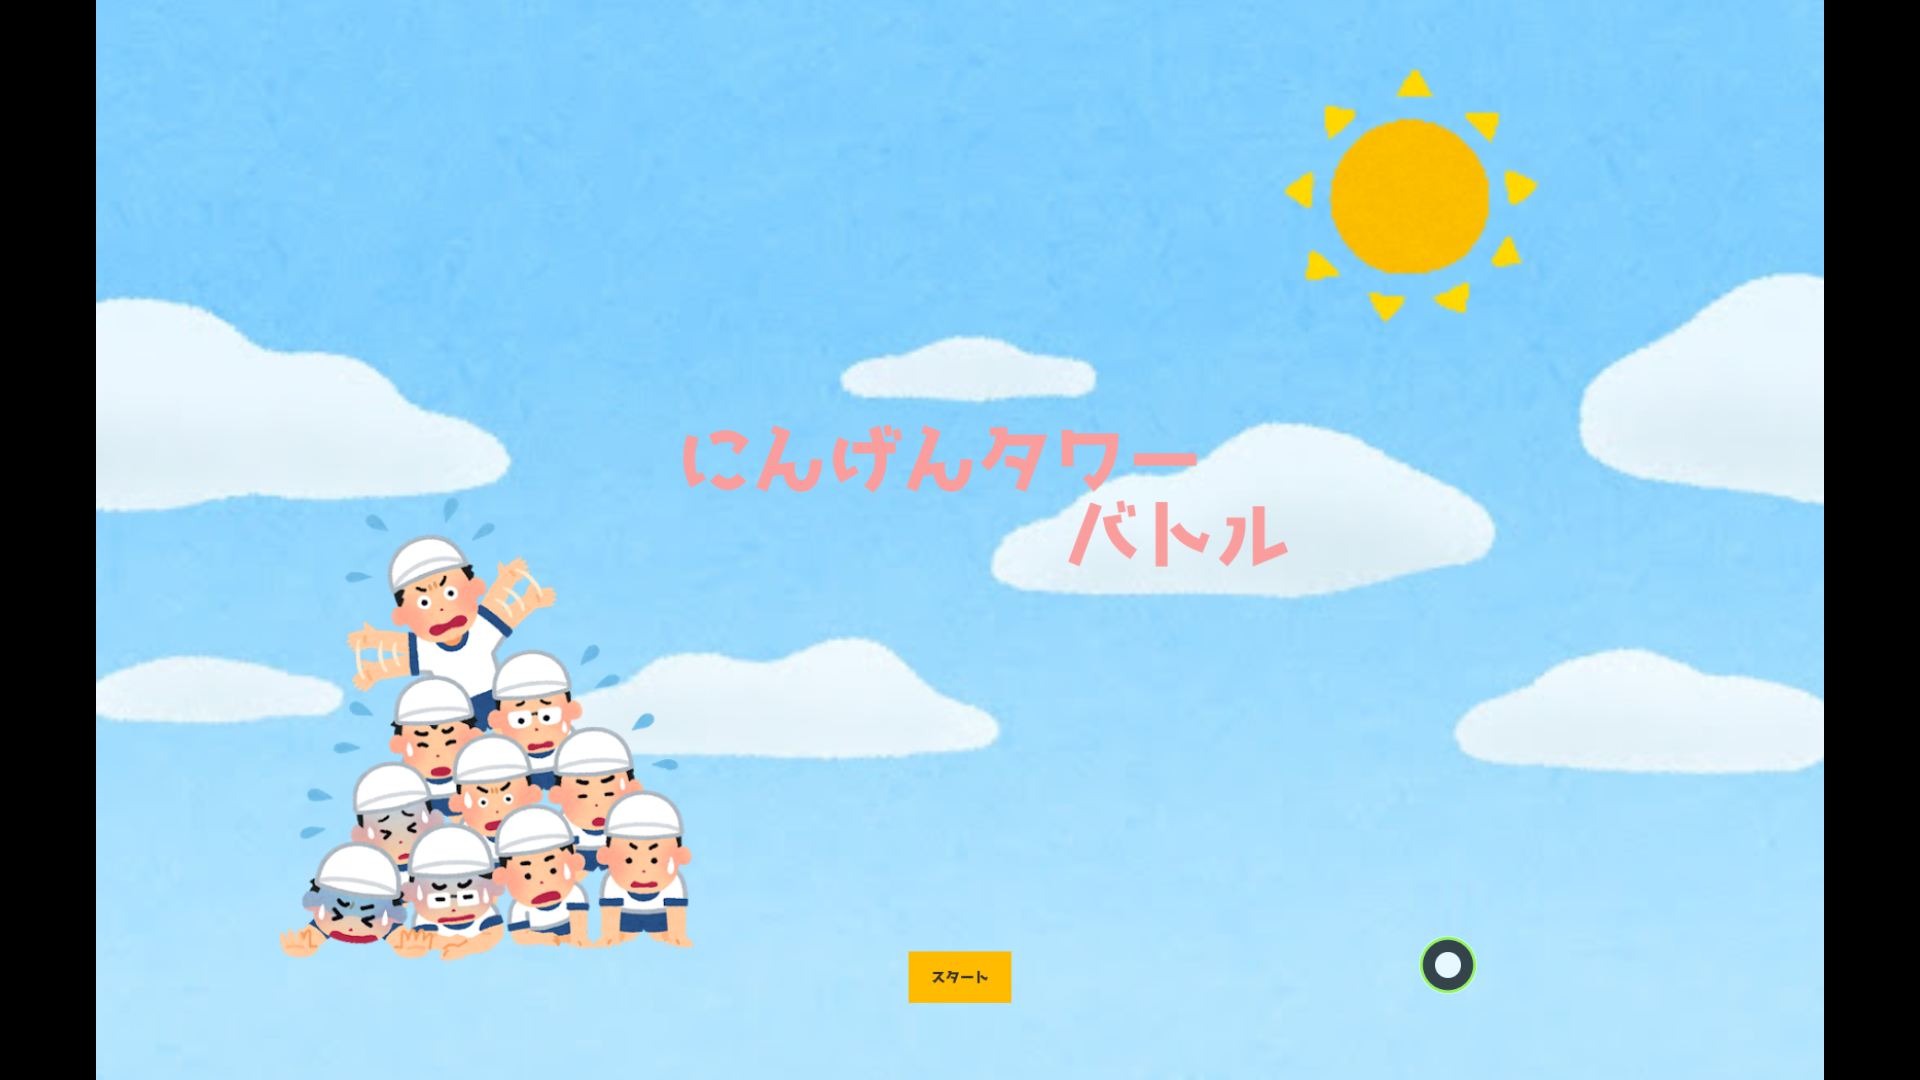
\includegraphics[keepaspectratio, scale=0.2]
  {images/startgame.png}
  \subcaption{スタート画面}\label{start}
 \end{minipage}
 \\
 \begin{minipage}[b]{0.5\linewidth}
  \centering
  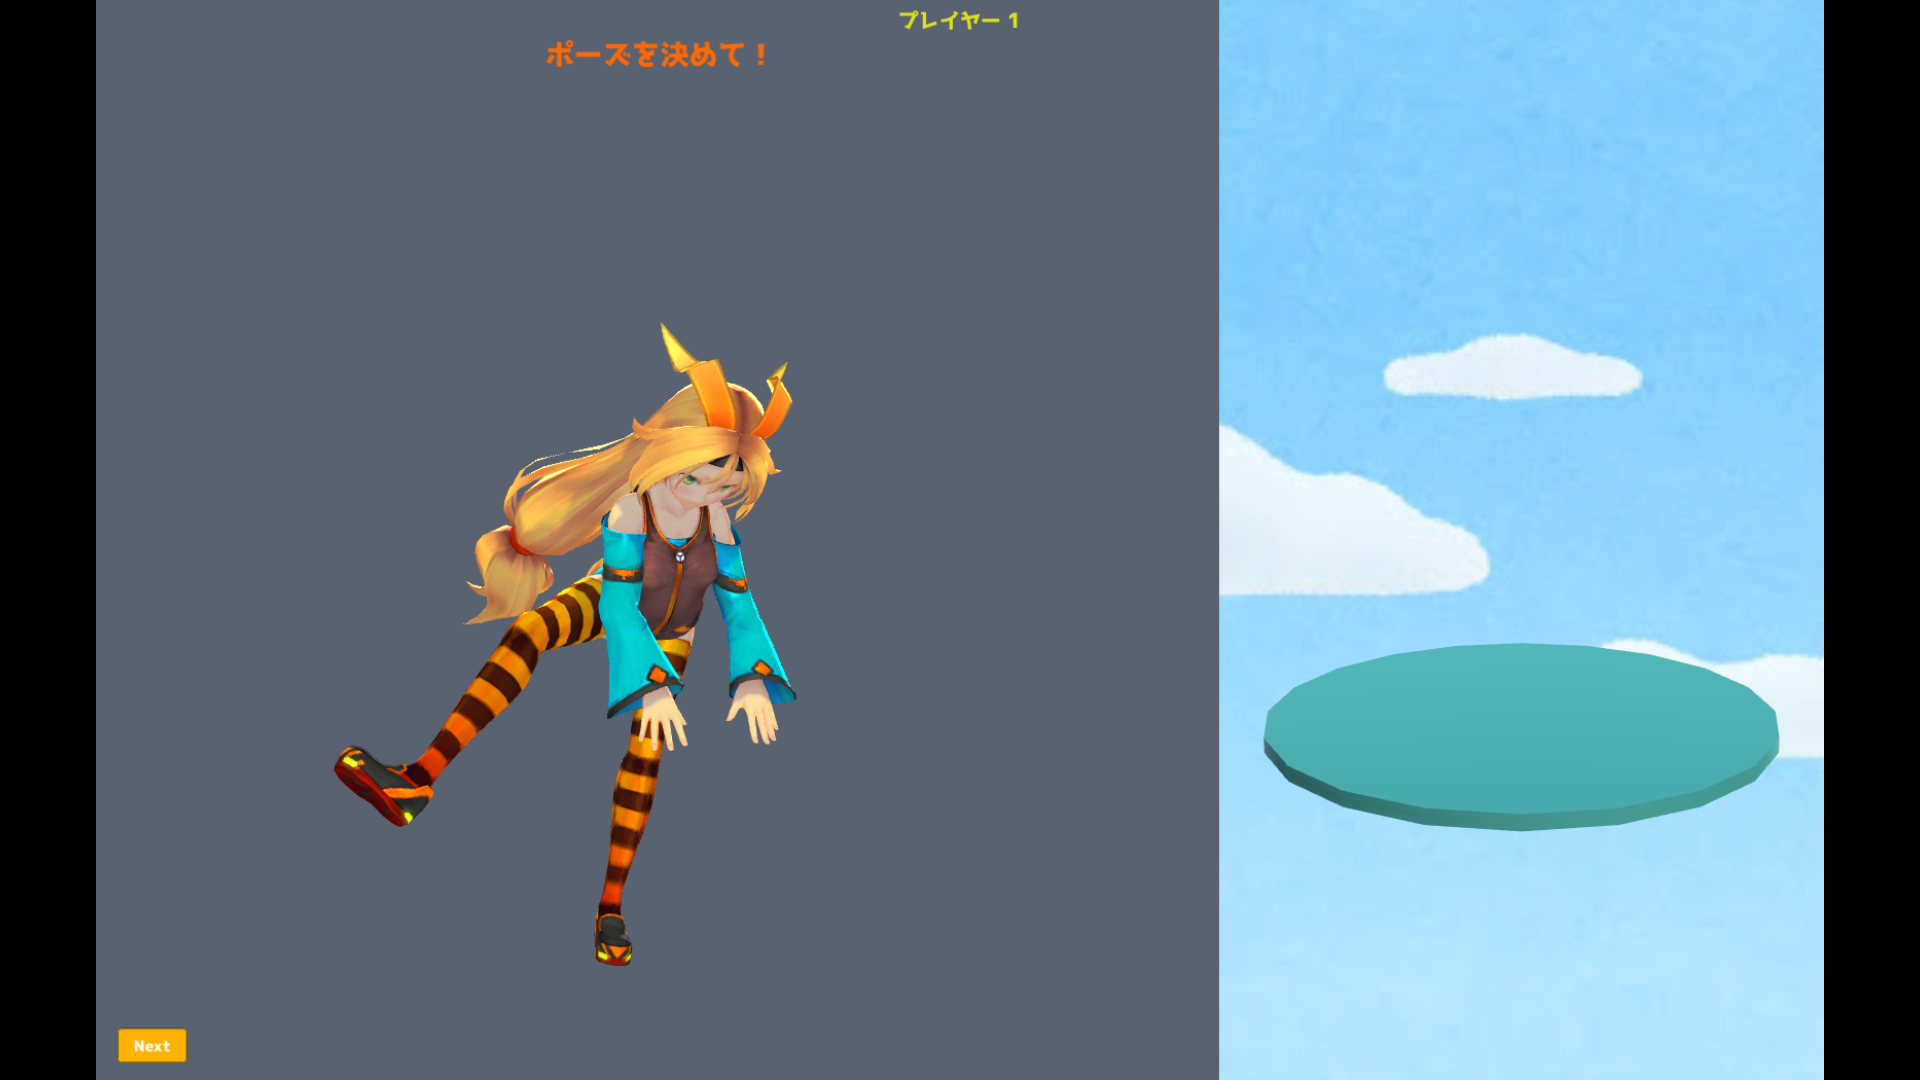
\includegraphics[keepaspectratio, scale=0.2]
  {images/game4.png}
  \subcaption{ポーズを決める画面}\label{pose}
 \end{minipage}
\\
 \begin{minipage}[b]{0.5\linewidth}
  \centering
  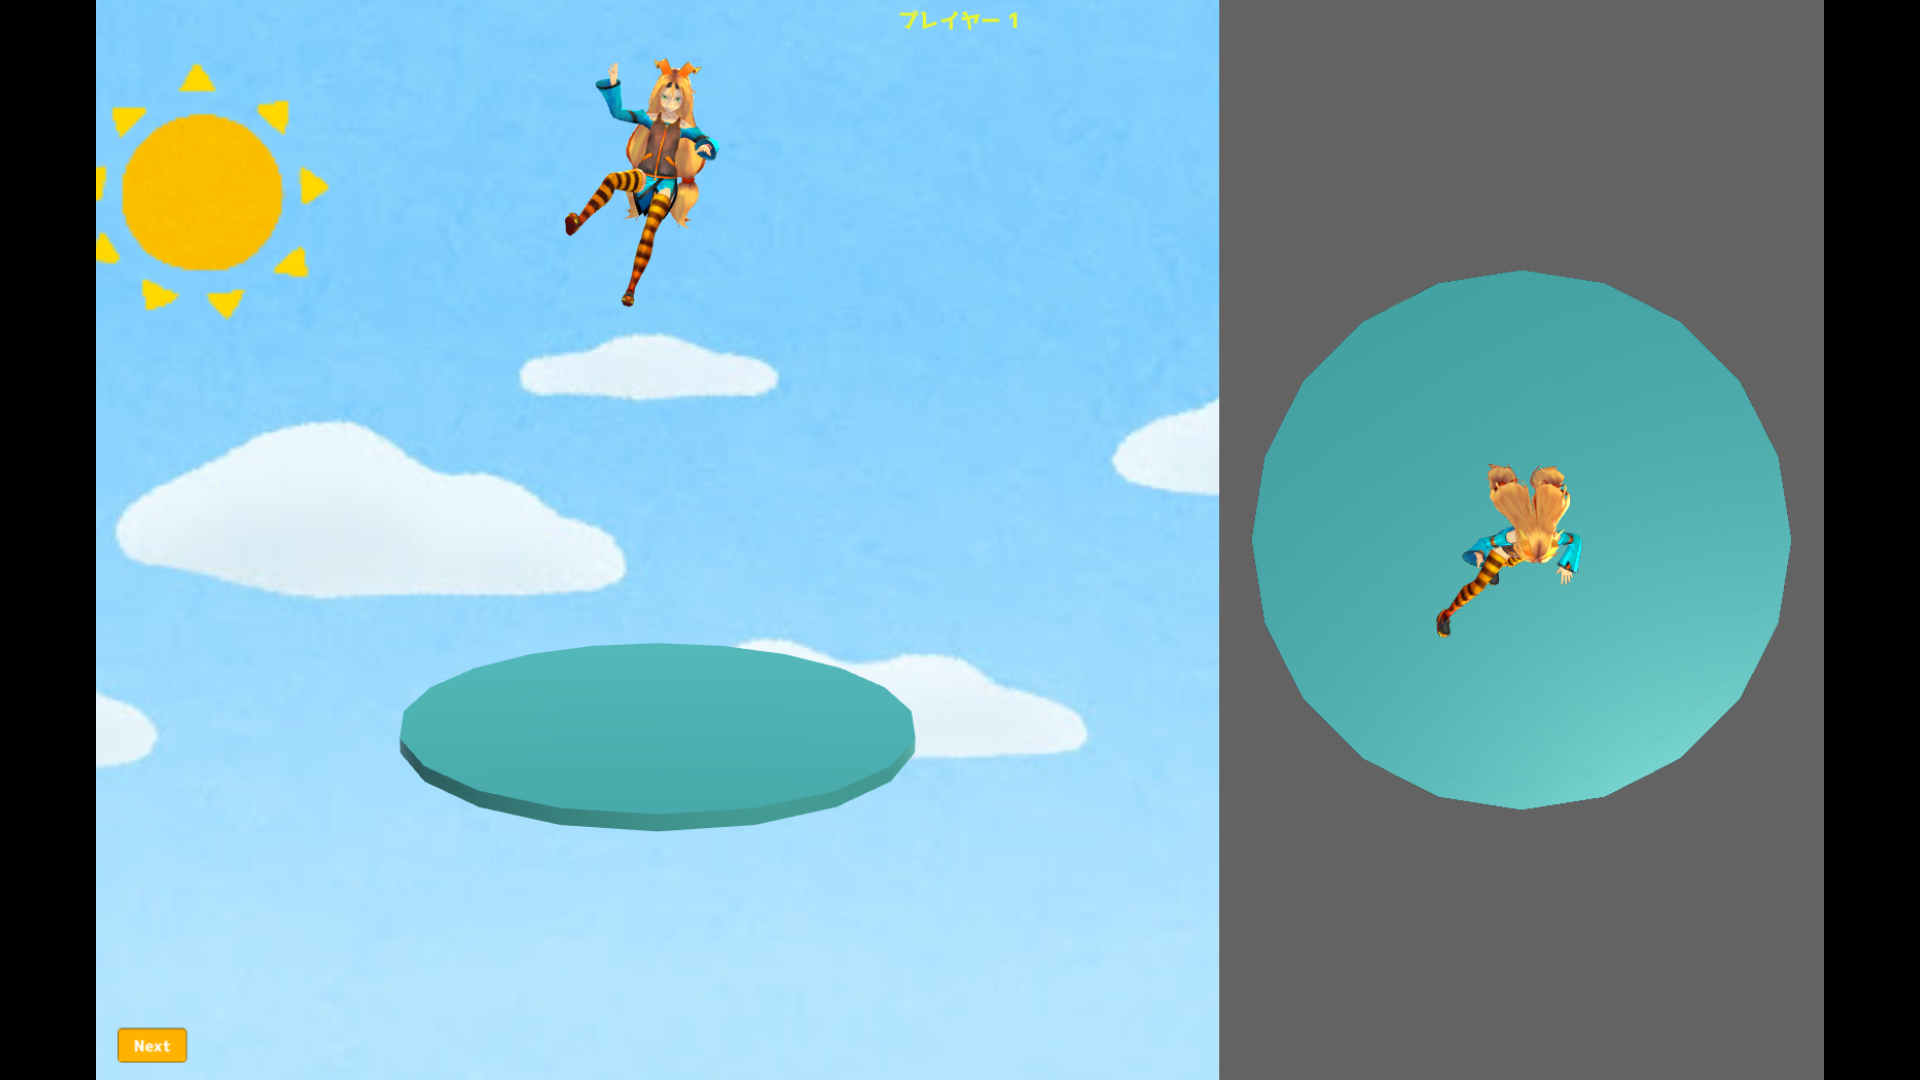
\includegraphics[keepaspectratio, scale=0.2]
  {images/game2.png}
  \subcaption{落とす位置と姿勢を決める画面1}\label{position1}
 \end{minipage}
 \end{figure}
 \begin{figure}
 \begin{minipage}[b]{0.5\linewidth}
  \centering
  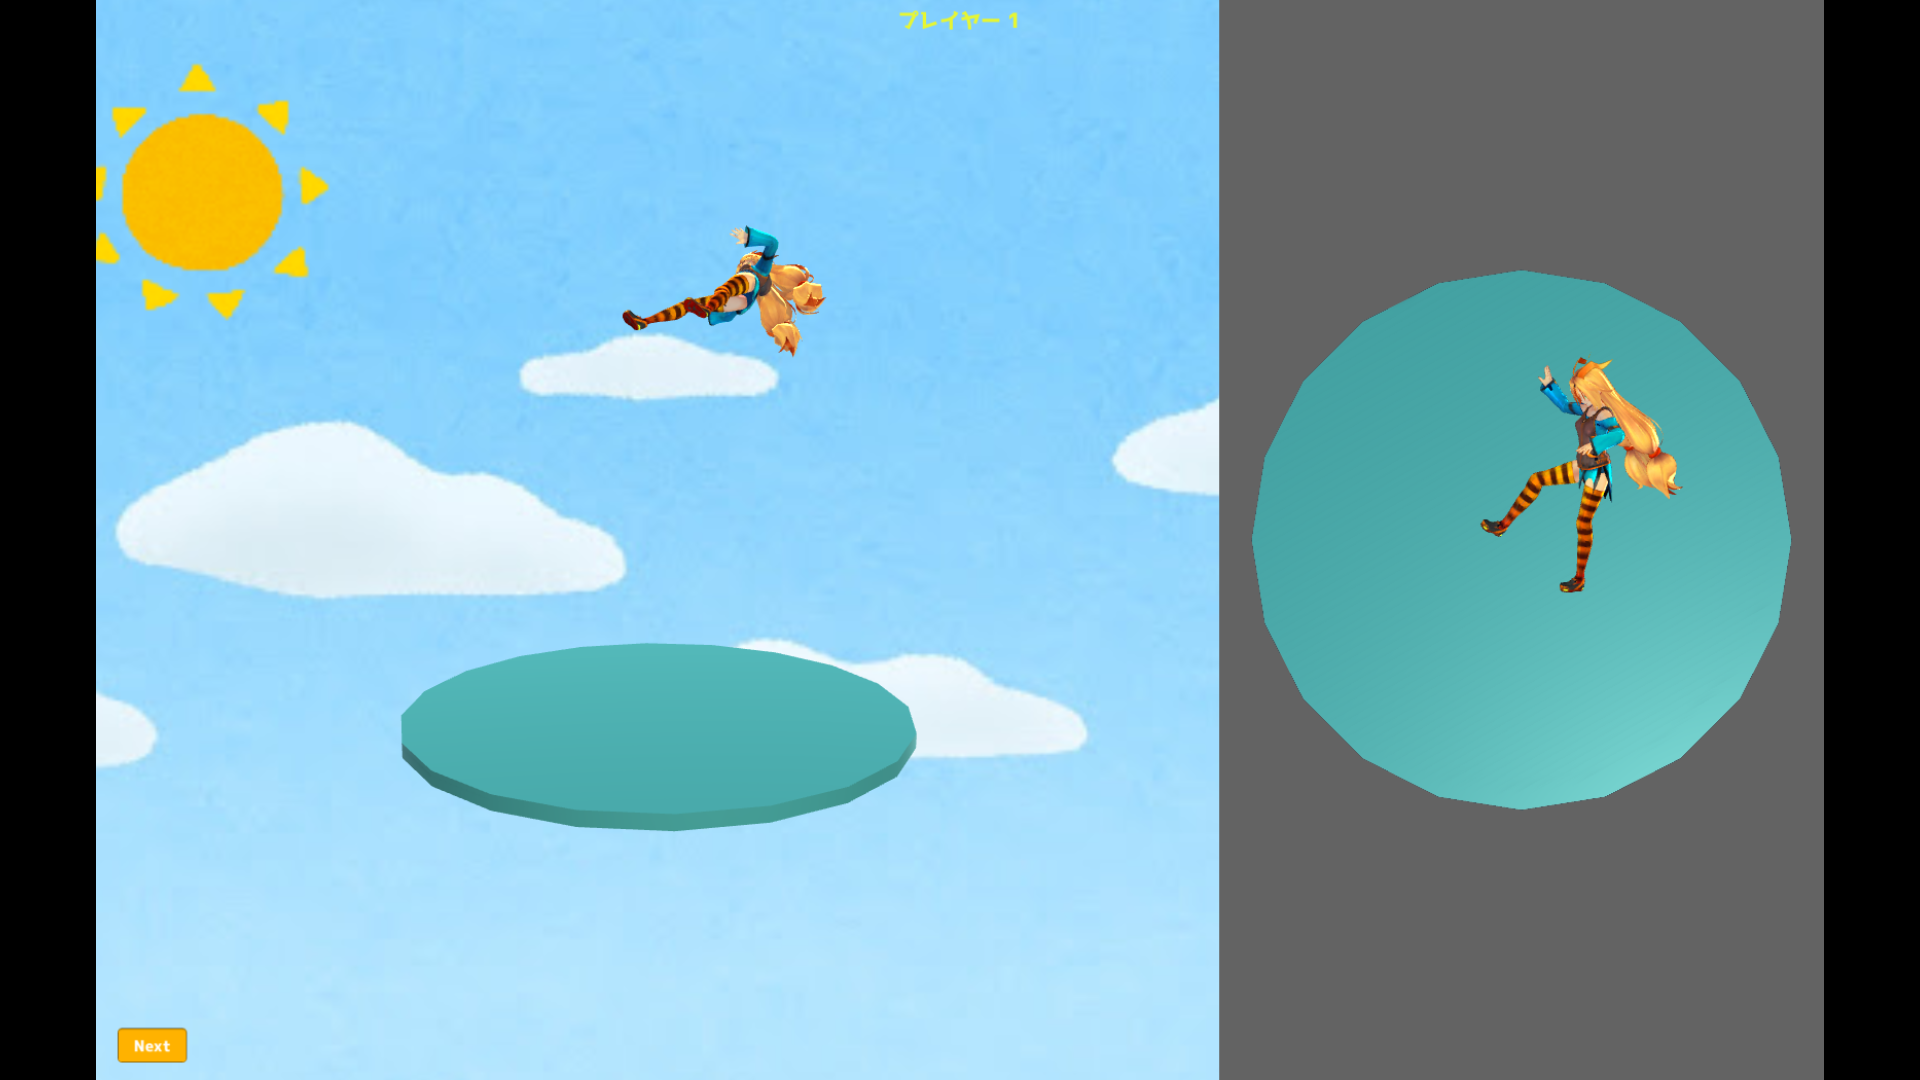
\includegraphics[keepaspectratio, scale=0.2]
  {images/game3.png}
  \subcaption{落とす位置と姿勢を決める画面2}\label{position2}
 \end{minipage}
 \\
 \begin{minipage}[b]{0.5\linewidth}
  \centering
  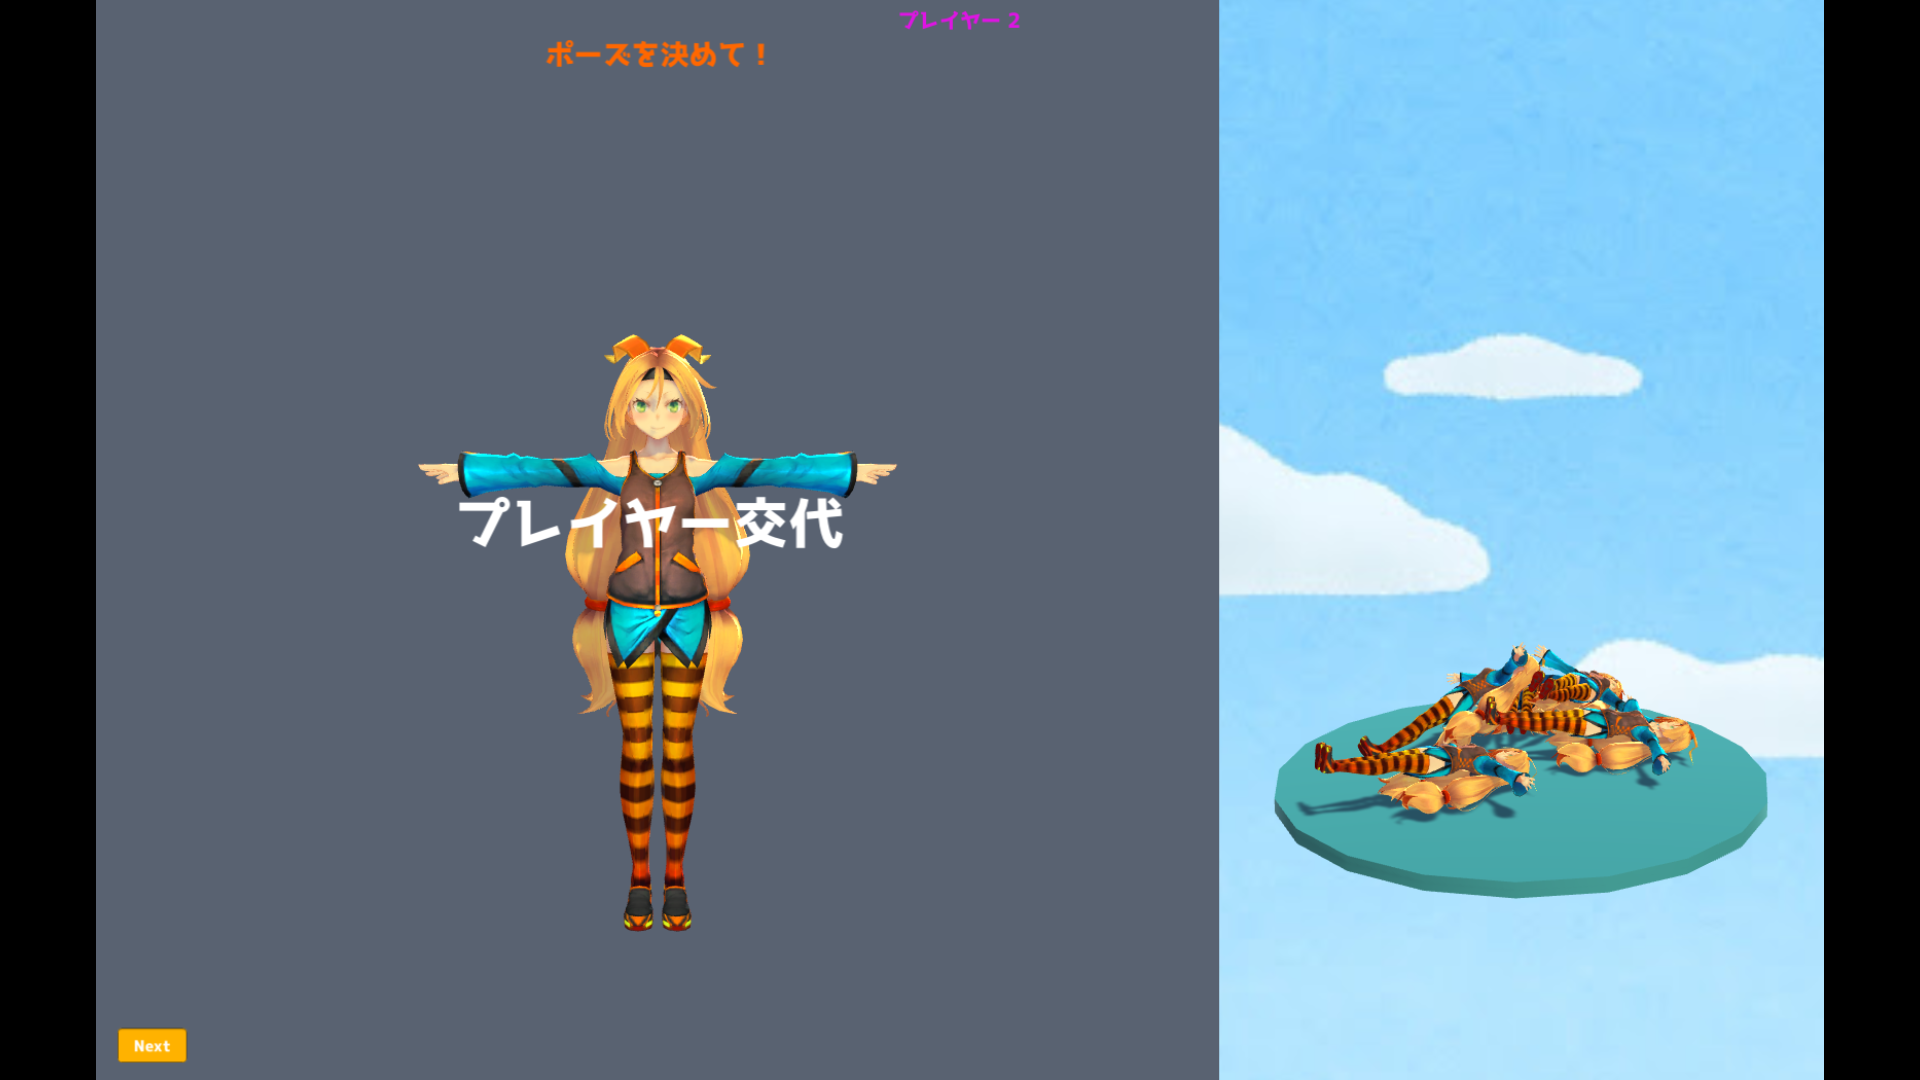
\includegraphics[keepaspectratio, scale=0.2]
  {images/game5.png}
  \subcaption{何度か積み重ねていった画面}\label{tumi}
 \end{minipage}
 \caption{ゲーム画面}\label{game}
\end{figure}



\section{今後改善したい点・自主プロジェクトの感想}
今回肝心の骨格推定からunityの人形に落とし込むということをアセットを用いで実現させたため,そのプログラムを少しだけ書き換えるということしか行わなかった.恐らく一から自力でこの過程をプログラムするとなると自主プロ期間内では間に合わなかったため断念したのだが,春休みに時間があるのではじめに断念したopenposeを用いて骨格推定を行いそれをunityにうまく落とし込むことをやりたいと思う.また,時間がなかったため,人形
が1種類となってしまったが,3種類ほど(重くて反発係数が小さいキャラ,中くらいのキャラ,軽くて反発係数が大きいキャラ)のように重さや反発係数や摩擦係数や大きさなど様々な種類の人形を作るとより面白いゲームになりそうだと思ったのでブレンダーを用いて自分のキャラクターを作りたかった.

この自主プロジェクトを通して,他人の書いたプログラムを理解し自分の機能に合わせて
変更していくという能力が身についたと思う.今後は,そのようなプログラムを書き換えるのではなく一から作れるようになりたい.また,unityを用いるのは今回が初めてだったのだがunityについてかなり深くまで知ることができたのはとても良かった.春休みはunityを用いてまた別のゲーム(ARやVR)を作ってみたい.

\begin{thebibliography}{9}
\bibitem{openpose} tf-pose-estimation https://github.com/ildoonet/tf-pose-estimation
\bibitem{kinect} kinect v2 examples with ms-sdk  https://assetstore.unity.com/packages/3d/characters/kinect-v2-examples-with-ms-sdk-and-nuitrack-sdk-18708?aid=1011lGbg\&utm\_source=aff
\end{thebibliography}

\end{document}
